
\subsection{Trip Generation}

We had to rely on the Gravity Model of transportation planning in order to estimate the trip generation. However, we adjusted it to fit our needs. Since the end point of all trips was the same, we did not need the factor of $P_j$ and the model constant $K$ was just a normalizing factor to make the total number of trips from all zones equal to the total attendance. $K$ was calculated as $(T_{ij}/T_{total}) \times (\mathrm{Total attendance})$. The map below shows the results of the Gravity Model by displaying the number of trips originating from each zip code to the stadium.

\begin{figure}[htp]
  \centering
  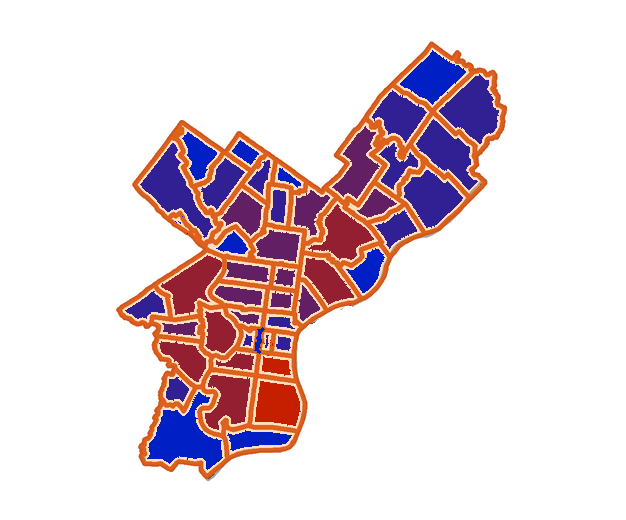
\includegraphics[height=8cm]{graphics/trip-generation.png}
  \caption{Map showing number of fans per zipcode}
  \label{fig-trip-generation-results}
\end{figure}

Looking at the results of the Gravity Model we can tell that …

For more accuracy we could include more factors in the model such as  average income of the people living in the zone. We could also use actual fan data, which we would need to obtain from the Phillies.


\subsection{Trip Distribution}

Trip Distribution data needs to be researched. The SEPTA website has a Revenue and Ridership Report that gives trip distribution throughout the day and also average daily ridership, which we can combine and extrapolate to produce the average number of people riding per minute throughout the day. Shown below is the trip distribution bar graph provided in the February 2013 Revenue and Ridership Report:

\begin{figure}[htp]
  \centering
  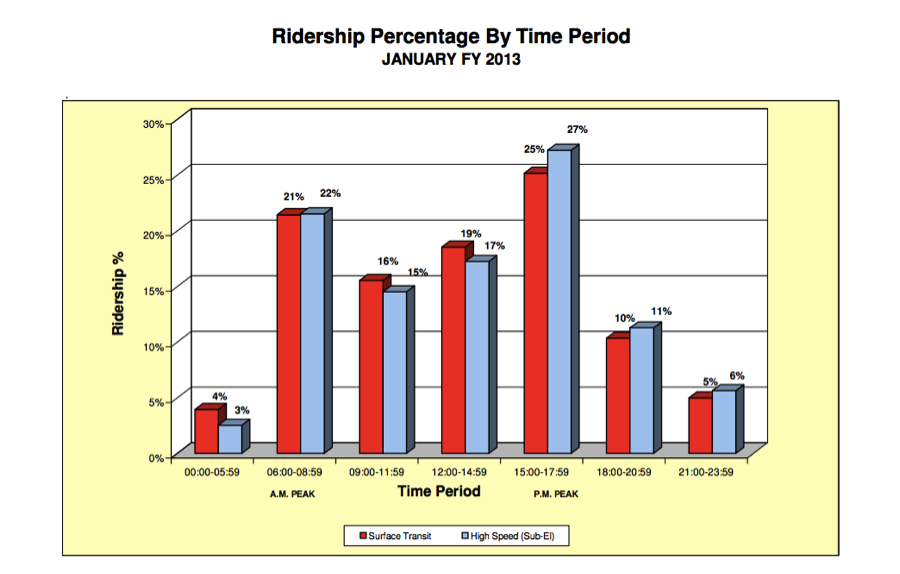
\includegraphics[height=7cm]{graphics/ridership-per-period.png}
  \caption{Average Daily Ridership By Time Period}
  \label{fig-ridership-per-period}
\end{figure}

Furthermore, we used data from a stadium planning study called Traffic Operations Planning for Stadia and Arenas in order to obtain the distribution of trips going to a stadium. Below is the table we obtained:

\begin{table}
  \centering
  \begin{tabular}{cc}
    Minutes to Game Time & Percentage of Crowd \\
    \hline\hline
    -60 minutes & 24\% \\
    -40 minutes & 38\% \\
    -20 minutes & 54\% \\
     Game Time  & 72\% \\
    +20 minutes & 82\% \\
    +40 minutes & 92\% \\
    +60 minutes & 100\% \\
  \end{tabular}
  \caption{Cumulative arrivals to stadium as a percentage of total crowd (45,000 fans)}
  \label{tab-arrivals}
\end{table}

This table gives us the trip distribution for the trips that we generated from the Trip Generation Gravity Model.


\subsection{Mode Choice}

As we had planned, we were able to obtain both parking lot data from the Philadelphia Phillies, as well as average ridership data from SEPTA. We found out that there were on average 7,400 trips per game on SEPTA. Additionally, we found out there are typically 17,000 cars parked in the parking lots every game. We found that if back-out the average number of passengers per car we get 2, which has been cross-referenced with traffic data for the United States. In order to back out the number we assume 95\% occupancy of 43,651, or 41,468 total fans. We then removed the number of people taking SEPTA, which gives us 34,068. Then divide that by the number of cars, which gives us 2.

